\item $f(x) = 2\cdot\sin\left(-3(x+\frac{1}{6}\pi)\right)+1$

Die Periode ist $\frac{2}{3}\pi$. Die Nullage ist bei $1$, die Amplitude $2$. Zuerst wird mit Faktor $3$ entlang x-Richtung gestaucht, dann an der y-Achse gespiegelt und dann um $\frac{1}{6}\pi$ nach links verschoben. $\frac{1}{6}\pi$ entspricht $\frac{1\pi}{6} / \frac{2\pi}{3} = 1/4$ Periode. Bei $x=0$ ist also ein Minimum.

\begin{center}
  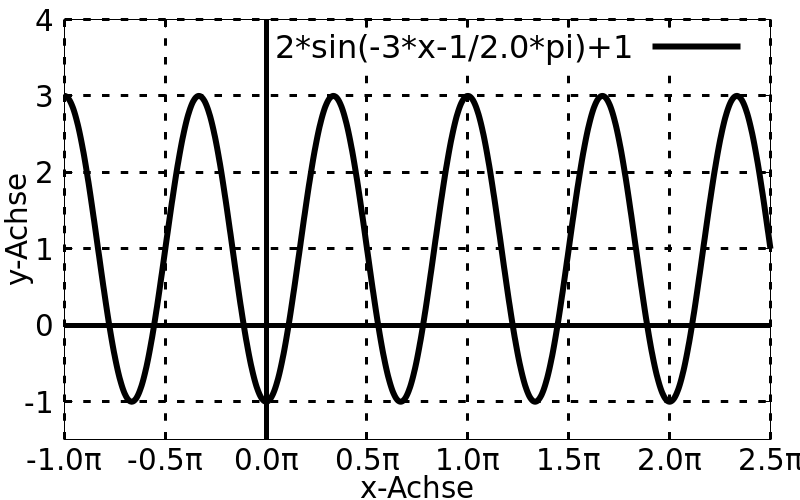
\includegraphics[width=0.95\textwidth]{../tex-snippets/ex-fn-transform-5-a.png}
\end{center}

